\documentclass{article}
\usepackage{indentfirst}  % Adds indentation to the first paragraph of each section
\usepackage{amsmath}      % Provides additional math symbols
\usepackage{amssymb}      % Provides \mathbb for blackboard bold symbols
\usepackage{hyperref}     % For hyperlinks in the bibliography
\usepackage{stmaryrd}
\usepackage{tikz}
\usetikzlibrary{3d}

\setlength{\parindent}{15pt}  % Adjust the size of the paragraph indent
\linespread{1.5}  % Set line spacing to 1.5 times

\begin{document}

\section*{Chapter I: Application of the theory of conceptual spaces to colours}

\hspace*{\parindent}A colour space is used to represent the three-dimensional organisation of colours. Colours are mapped along axes that represent different colour properties. A first example is the space $\mathbf{RGB}$ whose three dimensions represent red, green, and blue respectively.

A singular colour shade is represented in $\mathbf{RGB}$ by a triplet\footnote{This space is often used in computing, where the value of red, green and blue is encoded by a byte that can have 256 different values.} $\left(x_1,x_2,x_3\right) \in \left(R \times G \times B\right)$ where $R \times G \times B = \llbracket 0 ; 255 \rrbracket \times \llbracket 0 ; 255 \rrbracket \times \llbracket 0 ; 255 \rrbracket \subset \mathbb{N}^3$. Intuitively, this triplet represents the level of red, green, and blue in the singular colour shade.

More generally, the $\mathbf{RGB}$ space models each colour shade as an additive combination of its value over the three dimensions of red, green, and blue. $\mathbf{RGB}$ space can be represented by a cube, where each axis represents the intensity of the components: red, green, and blue.

Although the \textbf{RGB} space has the merit of being simple, we will present two schematic ideas that show that it is not at all suitable for modelling human vision. Firstly, since the dimensions of \textbf{RGB} are chromatic, brightness information must be extracted from the three components encoding chromaticity. However, to model the human visual system, it is more appropriate to isolate a brightness parameter from the chromaticity parameters \cite[p.78]{fairchild2013}. The second criticism concerns the opposite colours in \textbf{RGB}. When space \textbf{RGB} is represented as a cube, it appears that each vertex — which intuitively corresponds to a 'pure colour' — has an opposite vertex that is also the furthest away on the cube. In other words, the four diagonals joining the four opposite vertices on the cube indicate the four pairs of colours furthest apart (cf. Fig. 1a). Thus, one of the shortcomings of the \textbf{RGB} model is that the vertex opposite that of RED is the one corresponding to CYAN. However, during the nineteenth and twentieth centuries, a number of empirical studies and theories support the idea that the most opposite colour to RED is GREEN, and not CYAN as is the case in \textbf{RGB}.

Gärdenfors \cite[section 2.1]{gardenfors2014} presents the three-dimensional colour space \textbf{HSL}, comprising the dimensions of hue, saturation and luminosity. This model solves the two problems previously raised: firstly, it dissociates the luminosity dimension from the chromatic dimensions, and secondly, it separates RED and GREEN on the saturation axis as far as possible (see Fig. 1.b).

\begin{figure}[h]
\centering
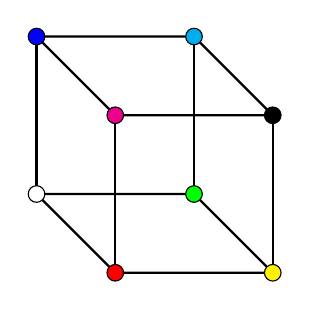
\begin{tikzpicture}[x={(0.5cm,-0.5cm)}, y={(1cm,0cm)}, z={(0cm,1cm)}]

% Define the coordinates of the cube
\coordinate (A) at (0,0,0);
\coordinate (B) at (2,0,0);
\coordinate (C) at (2,2,0);
\coordinate (D) at (0,2,0);
\coordinate (E) at (0,0,2);
\coordinate (F) at (2,0,2);
\coordinate (G) at (2,2,2);
\coordinate (H) at (0,2,2);

% Draw the back face
\draw[thick] (D) -- (C) -- (B) -- (A) -- cycle;

% Draw the front face
\draw[thick] (E) -- (F) -- (G) -- (H) -- cycle;

% Connect the front and back faces
\draw[thick] (A) -- (E);
\draw[thick] (B) -- (F);
\draw[thick] (C) -- (G);
\draw[thick] (D) -- (H);

% Add colored circles with black outlines at the vertices
\draw[black, fill=white] (A) circle (3pt);
\draw[black, fill=red] (B) circle (3pt);
\draw[black, fill=yellow] (C) circle (3pt);
\draw[black, fill=green] (D) circle (3pt);
\draw[black, fill=blue] (E) circle (3pt);
\draw[black, fill=magenta] (F) circle (3pt);
\draw[black, fill=black] (G) circle (3pt);
\draw[black, fill=cyan] (H) circle (3pt);

\end{tikzpicture}
\caption{RGB colour cube}
\label{fig:rgb_cube}
\end{figure}

\bibliographystyle{plain}
\bibliography{references}

\end{document}
